\documentclass[a4paper,11pt]{article}
 
\usepackage[english]{babel}
\usepackage[utf8x]{inputenc}
\usepackage[T1]{fontenc}
\usepackage{graphicx}
\usepackage{geometry}
\geometry{
		body={170mm,230mm},
		left=25mm,top=25mm,
		headheight=25mm,headsep=7mm,
		marginparsep=4mm,
		marginparwidth=20mm,
		footnotesep=50mm
}
\usepackage{enumitem}
\setlist{noitemsep}
\usepackage{amsmath}
\usepackage{amssymb}
\usepackage{mathabx}
\usepackage{tikz}
\usetikzlibrary{automata,positioning,arrows}
\usepackage{verbatim}
 
\title{INFO-F-403 Introduction to Language Theory and Compilation\\Project Part 1: \textsc{S-COBOL} Lexical Analyzer}
\author{\textsc{Delhaye} Quentin}
 
\begin{document}
\maketitle

%%%%%%%%
%%%%%%%%
\section{Presentation of the implementation}
The program is divided into three classes: \texttt{Main}, \texttt{LexicalAnalyzer} and \texttt{SymbolsTable}.
\subsection{\texttt{Main}}
This is the public executable class interacting with the user. It will ask him to enter a line
of \textsc{S-COBOL} code, will store it into a String \texttt{str}, and then will feed it to the lexical analyzer until
the String is empty. The lexical analyzer will return an array of two Strings, the first being the token to subtract
to \texttt{str}. If the token contains a special character from the point of view of the regular expression
(such as \texttt{*} or \texttt{(}, for example), those characters need to be escaped before the subtraction, and then
un-escaped after it to allow a clean output.
When \texttt{str} is finally empty, the class prints on the standard output all the token/lexical unit couples
sent back by the lexical analyzer.

This ends when the user stops entering code by simply hitting the \texttt{return} key
without entering anything. When he does that, the class asks the lexical analyzer to print the table
of symbols.

\subsection{\texttt{LexicalAnalyzer}}
This class receives a String \texttt{input} from the \texttt{Main} class. The first things it does with it
is checking if it is a comment: \texttt{input} is in a new line and it matches the following regex:
\verb|(\*|\texttt{|}\verb|/).*\n$|.

If it is not a comment, the method \texttt{nextToken} splits \texttt{input} at the spaces and submits the first
chunck at every regex or list until a match is found. If no match is found, the next piece of \texttt{input}
is concatenated using a space and submited again until a match is found or all the pieces have been put back
together.

The various test are the following:
\begin{itemize}
	\item \verb|^\.\n$|, \texttt{ouput} is the end of the line;
	\item contained in the list \texttt{keywords} which is formed from the exhaustive list.
		An other list, \texttt{units}, holds the corresponding lexical unit at the same index.
	\item \verb|^'[\w\ \-\+\*/:!\?]*'$|, String.
	\item \verb|0|\texttt{|}\verb|[\+\-]?[1-9][0-9]*|, integer.
	\item \verb|(0|\texttt{|}\verb|[\+\-]?[1-9][0-9]*)(\.[0-9]+)?|, real number. This regex is evaluated
		after the integer because a real number without a decimal part can be considered as a simple integer.
	\item \verb|s?9(\([1-9]\))?(v9(\([1-9]\))?)?|, image.
	\item \verb|^[a-zA-Z][\w\-]{0,14}|, identifier.
\end{itemize}

Each time an identifier is encountered, the token, as well as the line number on which it occurred,
are sent to the table of symbols.

Each time an image is encountered, if an identifier preceded it, they are both sent the the table of symbols.

If no valid token can be found in the input String, the lexical analyzer sends "\texttt{ERROR}" as a
lexical unit.


\subsection{\texttt{SymbolsTable}}
This class receives either variables or labels. In the first case, it must check if the identifier is
not already stored before saving it in the corresponding list. In the later case, it checks if the
identifier already is in the list, and if it is, if the line number is different. If the line number
is different, or if the identifier is brand new, the couple is apended to the list.

When the class is asked to format the list through the \texttt{toString} method, it first sorts both of the list
using the buble sort algorithm. The rest is just producing a String allowing a nice output.

\section{Hypothesis}
\begin{itemize}
	\item Each line is supposed to end with a \texttt{dot}.
	\item Every comments occupy full line and begin with \verb|*| or \texttt{/}.
	\item In order to avoid confusion, the user will leave space between the operands
		and the operators.
	\item Hyphenation is not allowed inside a String token.
\end{itemize}





\section{Automaton Reduction and Regular Expressions}

\subsection{Image}
The following will prove that the DFA shown at figure~\ref{DFA_image} can be reduced to
a regular expression. The transformation from a DFA into an RE will be achieved 
through state elimination.

\textit{Note:} \texttt{[1-9]} represents the range \texttt{[1;9]}


\begin{figure}[!h]
\centering
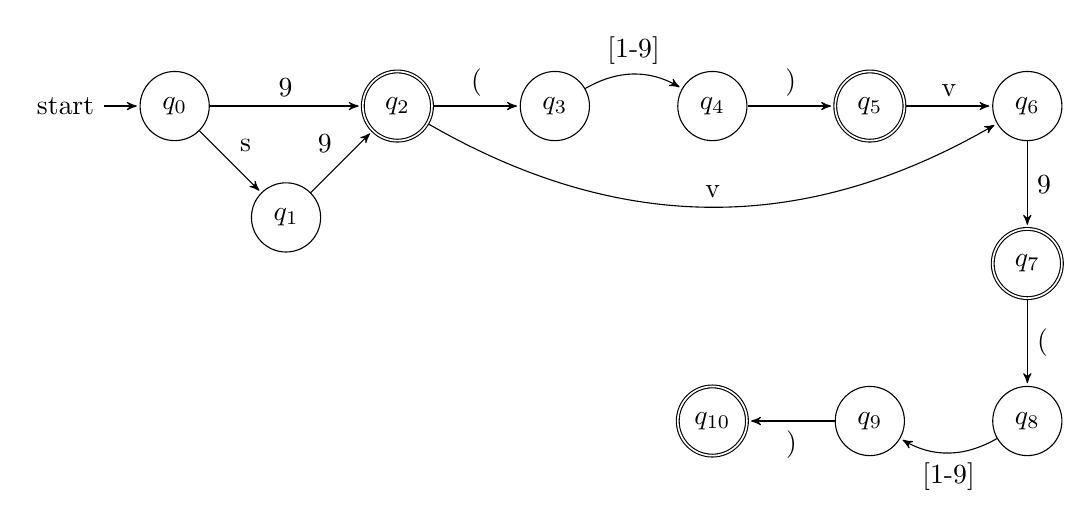
\begin{tikzpicture}[shorten >=1pt, node distance=2cm,on grid,auto,->, >=stealth']
	\node[state,initial](q_0){$q_0$};
	\node[state](q_1)[below right of=q_0]{$q_1$};
	\node[state,accepting](q_2)[above right of=q_1]{$q_2$};
	\node[state](q_3)[right of=q_2]{$q_3$};
	\node[state](q_4)[right of=q_3]{$q_4$};
	\node[state,accepting](q_5)[right of=q_4]{$q_5$};
	\node[state](q_6)[right of=q_5]{$q_6$};
	\node[state,accepting](q_7)[below of=q_6]{$q_7$};
	\node[state](q_8)[below of=q_7]{$q_8$};
	\node[state](q_9)[left of=q_8]{$q_9$};
	\node[state,accepting](q_10)[left of=q_9]{$q_{10}$};

	\path
	(q_0) edge 	node {s} (q_1)
	edge		node {9} (q_2)
	(q_1) edge 	node {9} (q_2)
	(q_2) edge 	node {(} (q_3)
	edge [bend right]	node {v} (q_6)
	(q_3) edge [bend left]	node {[1-9]} (q_4)
	(q_4) edge 	node {)} (q_5)
	(q_5) edge 	node {v} (q_6)
	(q_6) edge 	node {9} (q_7)
	(q_7) edge 	node {(} (q_8)
	(q_8) edge [bend left]	node {[1-9]} (q_9)
	(q_9) edge 	node {)} (q_10);
\end{tikzpicture}
\caption{DFA recognizing an image}
\label{DFA_image}
\end{figure}


\begin{itemize}
	\item $q_0 \rightarrow q_2$
	\begin{center}
	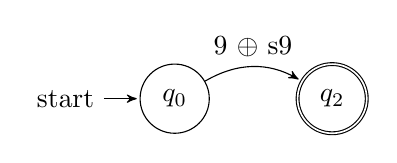
\begin{tikzpicture}[shorten >=1pt, node distance=2cm,on grid,auto,->, >=stealth']
		\node[state,initial](q_0){$q_0$};
		\node[state,accepting](q_2)[right of=q_0]{$q_2$};

		\path
		(q_0) edge [bend left] node {9 $\oplus$ s9} (q_2);
	\end{tikzpicture}
	\end{center}

	\item $q_0 \rightarrow q_5$
	\begin{center}
	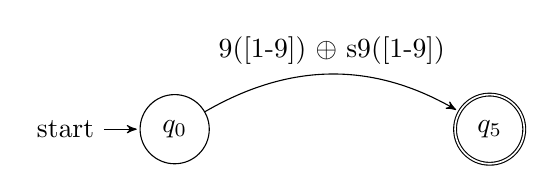
\begin{tikzpicture}[shorten >=1pt, node distance=4cm,on grid,auto,->, >=stealth']
		\node[state,initial](q_0){$q_0$};
		\node[state,accepting](q_5)[right of=q_0]{$q_5$};

		\path
		(q_0) edge [bend left] node {9([1-9]) $\oplus$ s9([1-9])} (q_5);
	\end{tikzpicture}
	\end{center}

	\item $q_0 \rightarrow q_7$
	\begin{center}
	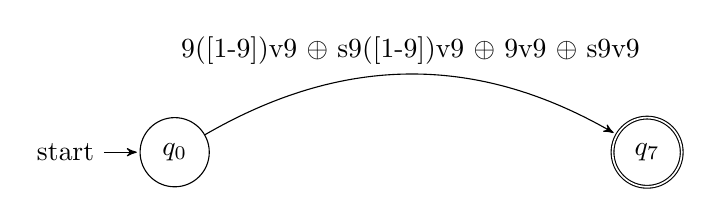
\begin{tikzpicture}[shorten >=1pt, node distance=6cm,on grid,auto,->, >=stealth']
		\node[state,initial](q_0){$q_0$};
		\node[state,accepting](q_7)[right of=q_0]{$q_7$};

		\path
		(q_0) edge [bend left] node {9([1-9])v9 $\oplus$ s9([1-9])v9 $\oplus$ 9v9 $\oplus$ s9v9} (q_7);
	\end{tikzpicture}
	\end{center}

	\item $q_0 \rightarrow q_{10}$
	\begin{center}
	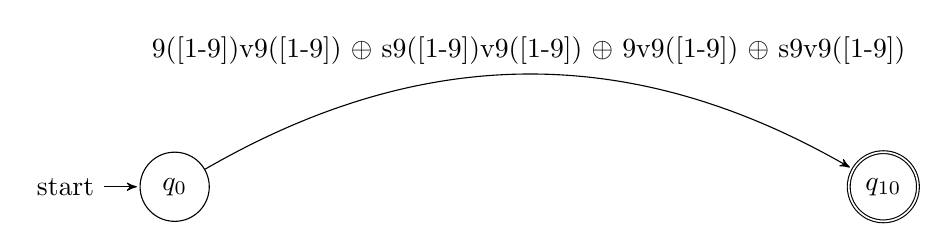
\begin{tikzpicture}[shorten >=1pt, node distance=9cm,on grid,auto,->, >=stealth']
		\node[state,initial](q_0){$q_0$};
		\node[state,accepting](q_10)[right of=q_0]{$q_{10}$};

		\path
		(q_0) edge [bend left] node {9([1-9])v9([1-9]) $\oplus$ s9([1-9])v9([1-9]) $\oplus$ 9v9([1-9]) $\oplus$ s9v9([1-9])} (q_10);
	\end{tikzpicture}
	\end{center}
\end{itemize}

The regular expression corresponding to the whole DFA is then:
\begin{equation}\nonumber
\begin{split}
RE = {9 \oplus s9} \oplus {9([1-9]) \oplus s9([1-9])} \oplus {9([1-9])v9 \oplus s9([1-9])v9 \oplus 9v9 \oplus s9v9} \\
	\oplus {9([1-9])v9([1-9]) \oplus s9([1-9])v9([1-9]) \oplus 9v9([1-9]) \oplus s9v9([1-9])}
\end{split}
\end{equation}
~\\

Knowing that $(A \oplus AB) = A(\epsilon \oplus B)$, we have:
\begin{equation}\nonumber
\begin{split}
	RE = \ldbrack\{\epsilon \oplus s\}9\rdbrack \oplus \ldbrack\{\epsilon \oplus s\}9([1-9])\rdbrack 
	\oplus \ldbrack\{\epsilon \oplus s)9([1-9])v \oplus \{\epsilon \oplus s)9v\rdbrack9 \\
	\oplus \ldbrack\{\epsilon \oplus s\}9([1-9])v \oplus \{\epsilon \oplus s\}9v\rdbrack9([1-9]) \\
\end{split}
\end{equation}
\[\Leftrightarrow RE = \{\epsilon \oplus s\}9 \ldbrack\epsilon \oplus \{\epsilon \oplus ([1-9])\} \oplus \{([1-9])v \oplus v\}9
\oplus \{([1-9])v \oplus v\}9([1-9])\rdbrack\]
\[\Leftrightarrow RE = \{\epsilon \oplus s\}9 \ldbrack\epsilon \oplus \{\epsilon+([1-9])\}
\oplus \{([1-9])v \oplus v\}9\{\epsilon \oplus ([1-9])\}\rdbrack\]
\[\Leftrightarrow RE = \{\epsilon \oplus s\}9 \ldbrack\epsilon \oplus \{\epsilon \oplus ([1-9])\}
\oplus \{([1-9]) \oplus \epsilon\}v9\{\epsilon \oplus ([1-9])\}\rdbrack\]
~\\

Using the fact that $A \oplus \epsilon = \epsilon \oplus A$, we find:
\[ RE = \{\epsilon \oplus s\}9 \ldbrack\epsilon \oplus \{\epsilon \oplus ([1-9])\}
\{\epsilon \oplus v9\{\epsilon \oplus ([1-9])\}\}\rdbrack\]
~\\

According to the extended regular expressions, \texttt{$\epsilon \oplus A$} corresponds to
\texttt{$A?$}. Using that relation, we can deduce the following expression:
\begin{center}
	\texttt{s?9([1-9]?(v9[1-9]?)?)?}
\end{center}


%%%%%%%%%%%%%%%%%%%%
\subsection{Integer}
\begin{figure}[!h]
\centering
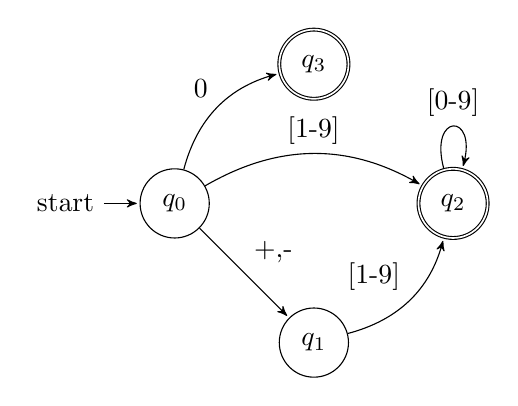
\begin{tikzpicture}[shorten >=1pt, node distance=2.5cm,on grid,auto,->, >=stealth']
	\node[state,initial](q_0){$q_0$};
	\node[state](q_1)[below right of=q_0]{$q_1$};
	\node[state,accepting](q_2)[above right of=q_1]{$q_2$};
	\node[state,accepting](q_3)[above right of=q_0]{$q_3$};

	\path
	(q_0) edge node {+,-}(q_1)
		edge [bend left] node {[1-9]} (q_2)
		edge [bend left] node {0}(q_3)
	(q_1) edge [bend right] node {[1-9]}(q_2)
	(q_2) edge [loop above] node {[0-9]}();
\end{tikzpicture}
\caption{Automaton recognizing an integer}
\end{figure}

\begin{itemize}
	\item $q_0 \rightarrow q_2$
	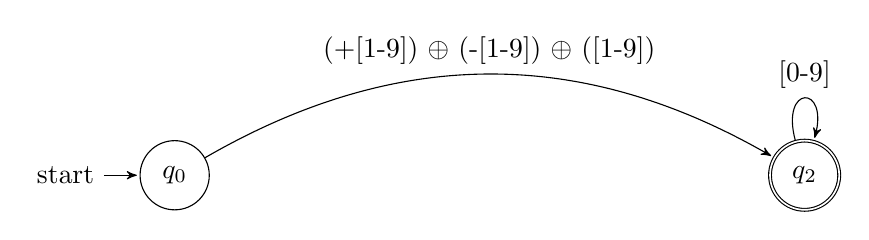
\begin{tikzpicture}[shorten >=1pt, node distance=8cm,on grid,auto,->, >=stealth']
		\node[state,initial](q_0){$q_0$};
		\node[state,accepting](q_2)[right of=q_0]{$q_2$};

		\path
		(q_0) edge [bend left] node {(+[1-9]) $\oplus$ (-[1-9]) $\oplus$ ([1-9])}(q_2)
		(q_2) edge [loop above] node {[0-9]} ();
	\end{tikzpicture}

\end{itemize}

\begin{equation}\nonumber
	RE = \ldbrack(+[1-9]) \oplus (-[1-9]) \oplus ([1-9])\rdbrack \oplus \ldbrack(+[1-9]) \oplus (-[1-9]) \oplus ([1-9])\rdbrack [0-9]^{*}
\end{equation}
\begin{equation}\nonumber
	\Leftrightarrow RE = \ldbrack(+[1-9]) \oplus (-[1-9]) \oplus ([1-9])\rdbrack \ldbrack\epsilon \oplus [0-9]^{*}\rdbrack
\end{equation}
\begin{equation}\nonumber
	\Leftrightarrow RE = \ldbrack+ \oplus - \oplus \epsilon\rdbrack[1-9] \ldbrack\epsilon \oplus [0-9]^*\rdbrack
\end{equation}
~\\

Since \texttt{a $\oplus$ b} is equivalent to the extended regular expression \texttt{[ab]}, we have:
\begin{center}
	\texttt{0 | [+-]?[1-9][0-9]*}
\end{center}

%%%%%%%%%%%%%%%%%
\subsection{Real}

\begin{figure}[!h]
\centering
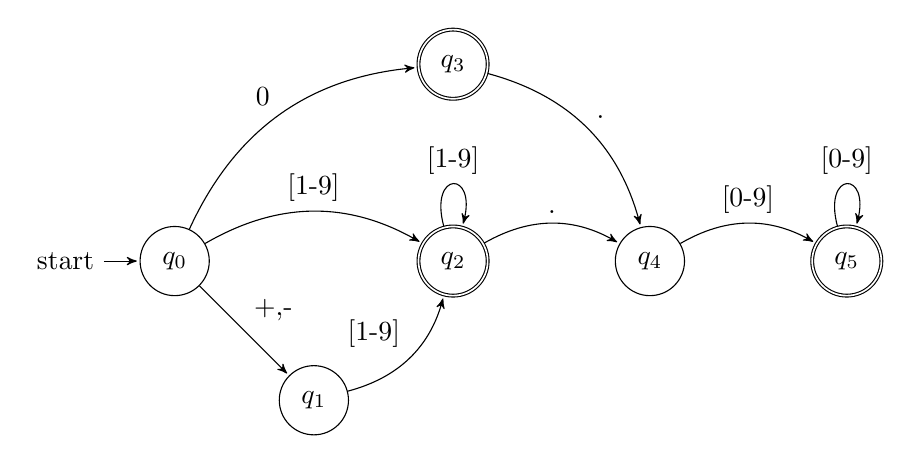
\begin{tikzpicture}[shorten >=1pt, node distance=2.5cm,on grid,auto,->, >=stealth']
	\node[state,initial](q_0){$q_0$};
	\node[state](q_1)[below right of=q_0]{$q_1$};
	\node[state,accepting](q_2)[above right of=q_1]{$q_2$};
	\node[state,accepting](q_3)[above of=q_2]{$q_3$};
	\node[state](q_4)[right of=q_2]{$q_4$};
	\node[state,accepting](q_5)[right of=q_4]{$q_5$};

	\path
	(q_0) edge node {+,-}(q_1)
	edge [bend left] node {[1-9]} (q_2)
		edge [bend left] node {0} (q_3)
		(q_1) edge [bend right] node {[1-9]}(q_2)
		(q_2) edge [loop above] node {[1-9]}()
		edge [bend left] node {.} (q_4)
	(q_3) edge [bend left] node {.} (q_4)
	(q_4) edge [bend left] node {[0-9]} (q_5)
	(q_5) edge [loop above] node {[0-9]} ();
\end{tikzpicture}
\caption{Automaton recognizing a real}
\end{figure}
\begin{itemize}
	\item $q_0 \rightarrow q_2$
		Same result as for the integer.

	\item $q_0 \rightarrow q_6$
	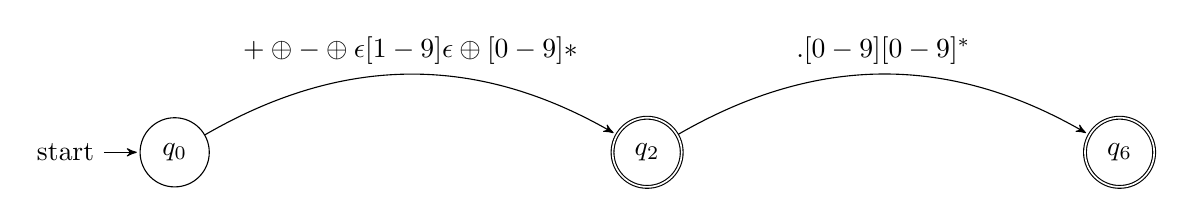
\begin{tikzpicture}[shorten >=1pt, node distance=6cm,on grid,auto,->, >=stealth']
		\node[state,initial](q_0){$q_0$};
		\node[state,accepting](q_2)[right of=q_0]{$q_2$};
		\node[state,accepting](q_6)[right of=q_2]{$q_6$};

		\path
		(q_0) edge [bend left] node {$\ldbrack+ \oplus - \oplus \epsilon\rdbrack[1-9] \ldbrack\epsilon \oplus [0-9]*\rdbrack$}(q_2)
		(q_2) edge [bend left] node {$.[0-9][0-9]^*$} (q_6);
	\end{tikzpicture}
\end{itemize}


\begin{equation}\nonumber
	RE = \ldbrack+ \oplus - \oplus \epsilon\rdbrack[1-9] \ldbrack\epsilon \oplus [0-9]^*\rdbrack \\
	\oplus \ldbrack+ \oplus - \oplus \epsilon\rdbrack[1-9] \ldbrack\epsilon \oplus [0-9]^*\rdbrack .[0-9][0-9]^*
\end{equation}
\begin{equation}\nonumber
	\Leftrightarrow RE = \ldbrack+ \oplus - \oplus \epsilon\rdbrack[1-9] \ldbrack\epsilon \oplus [0-9]*\rdbrack \\
		\oplus \ldbrack \epsilon \oplus .[0-9][0-9]^* \rdbrack
\end{equation}

Knowing that \verb|AA*| is equivalent to the extended regular expression \texttt{A+}, we have:
\begin{center}
	\texttt{(0 | [+-]?[1-9][0-9]*)(.[0-9]+)?}
\end{center}


%%%%%%%%
%%%%%%%%
\section{Notes on the DFA}
It is to be noted that the DFA Simulator can't recognize the comma -- \texttt{,} --
nor the "end of line" character.

The rejecting state is label \texttt{ERROR}.

\end{document}


